\documentclass{article}
\usepackage[margin=1in]{geometry}
\usepackage{amsmath,amssymb,tikz,graphicx}
\pagestyle{empty}
\begin{document}
\tikzset{every picture/.style={line width=0.75pt}} %set default line width to 0.75pt   
\centering     
\resizebox{0.9\textwidth}{!}{

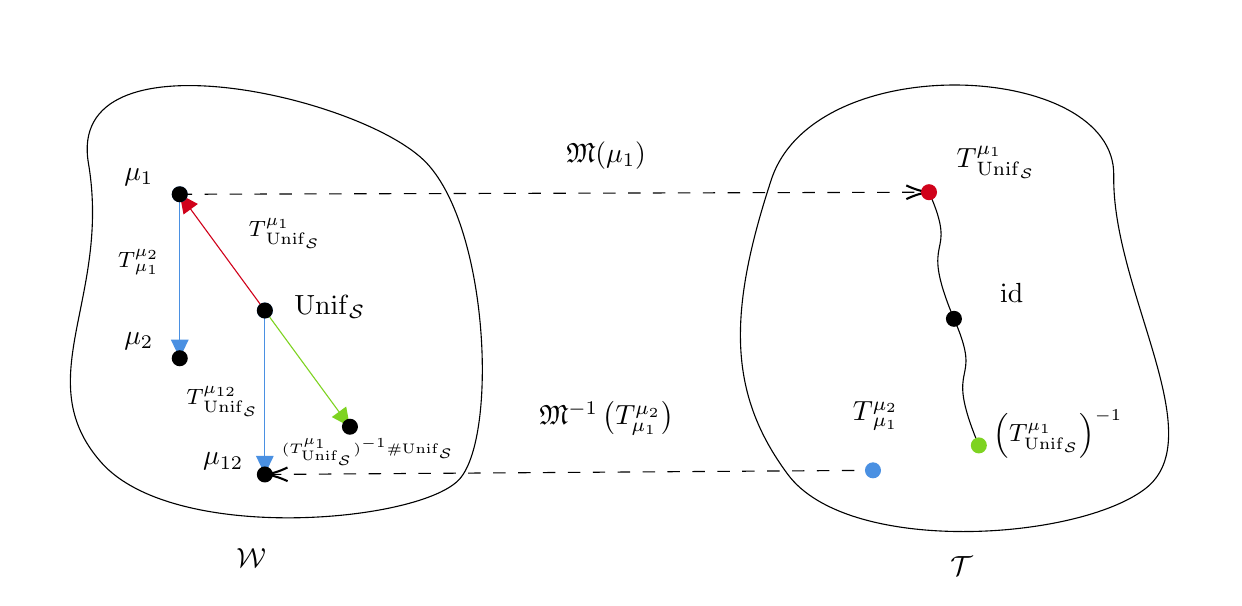
\begin{tikzpicture}[x=0.75pt,y=0.75pt,yscale=-1,xscale=1]
%uncomment if require: \path (0,300); %set diagram left start at 0, and has height of 300

%Straight Lines [id:da7336801203362149] 
\draw [color={rgb, 255:red, 126; green, 211; blue, 33 }  ,draw opacity=1 ]   (194.23,191.58) -- (155,138) ;
\draw [shift={(196,194)}, rotate = 233.79] [fill={rgb, 255:red, 126; green, 211; blue, 33 }  ,fill opacity=1 ][line width=0.08]  [draw opacity=0] (8.93,-4.29) -- (0,0) -- (8.93,4.29) -- cycle    ;
%Shape: Polygon Curved [id:ds3854113625849317] 
\draw   (70,67) .. controls (59,2) and (203,35) .. (233,67) .. controls (263,99) and (267,198) .. (249,219) .. controls (231,240) and (111,251) .. (76,211) .. controls (41,171) and (81,132) .. (70,67) -- cycle ;
%Shape: Polygon Curved [id:ds06891415618629226] 
\draw   (399,75) .. controls (420,11) and (565,18) .. (564,73) .. controls (563,128) and (612,199) .. (579,224) .. controls (546,249) and (436,256) .. (407,217) .. controls (378,178) and (378,139) .. (399,75) -- cycle ;
%Straight Lines [id:da14178531733745947] 
\draw [color={rgb, 255:red, 74; green, 144; blue, 226 }  ,draw opacity=1 ]   (155,138) -- (155,214) ;
\draw [shift={(155,217)}, rotate = 270] [fill={rgb, 255:red, 74; green, 144; blue, 226 }  ,fill opacity=1 ][line width=0.08]  [draw opacity=0] (8.93,-4.29) -- (0,0) -- (8.93,4.29) -- cycle    ;
\draw [shift={(155,138)}, rotate = 90] [color={rgb, 255:red, 74; green, 144; blue, 226 }  ,draw opacity=1 ][fill={rgb, 255:red, 74; green, 144; blue, 226 }  ,fill opacity=1 ][line width=0.75]      (0, 0) circle [x radius= 3.35, y radius= 3.35]   ;
%Straight Lines [id:da555203353595284] 
\draw [color={rgb, 255:red, 208; green, 2; blue, 27 }  ,draw opacity=1 ]   (155,138) -- (115.77,84.42) ;
\draw [shift={(114,82)}, rotate = 53.79] [fill={rgb, 255:red, 208; green, 2; blue, 27 }  ,fill opacity=1 ][line width=0.08]  [draw opacity=0] (8.93,-4.29) -- (0,0) -- (8.93,4.29) -- cycle    ;
%Straight Lines [id:da4627620747940214] 
\draw [color={rgb, 255:red, 74; green, 144; blue, 226 }  ,draw opacity=1 ]   (114,82) -- (114,158) ;
\draw [shift={(114,161)}, rotate = 270] [fill={rgb, 255:red, 74; green, 144; blue, 226 }  ,fill opacity=1 ][line width=0.08]  [draw opacity=0] (8.93,-4.29) -- (0,0) -- (8.93,4.29) -- cycle    ;
\draw [shift={(114,82)}, rotate = 90] [color={rgb, 255:red, 74; green, 144; blue, 226 }  ,draw opacity=1 ][fill={rgb, 255:red, 74; green, 144; blue, 226 }  ,fill opacity=1 ][line width=0.75]      (0, 0) circle [x radius= 3.35, y radius= 3.35]   ;
%Straight Lines [id:da3211782955741507] 
\draw    (114,161) ;
\draw [shift={(114,161)}, rotate = 0] [color={rgb, 255:red, 0; green, 0; blue, 0 }  ][fill={rgb, 255:red, 0; green, 0; blue, 0 }  ][line width=0.75]      (0, 0) circle [x radius= 3.35, y radius= 3.35]   ;
%Straight Lines [id:da32736082093249397] 
\draw    (155,217) ;
\draw [shift={(155,217)}, rotate = 0] [color={rgb, 255:red, 0; green, 0; blue, 0 }  ][fill={rgb, 255:red, 0; green, 0; blue, 0 }  ][line width=0.75]      (0, 0) circle [x radius= 3.35, y radius= 3.35]   ;
%Straight Lines [id:da9561895968401724] 
\draw  [dash pattern={on 4.5pt off 4.5pt}]  (114,82) -- (473,81.01) ;
\draw [shift={(475,81)}, rotate = 179.84] [color={rgb, 255:red, 0; green, 0; blue, 0 }  ][line width=0.75]    (10.93,-3.29) .. controls (6.95,-1.4) and (3.31,-0.3) .. (0,0) .. controls (3.31,0.3) and (6.95,1.4) .. (10.93,3.29)   ;
%Straight Lines [id:da304326169204612] 
\draw    (487,142) ;
%Straight Lines [id:da8234587689508922] 
\draw    (487,142) ;
\draw [shift={(487,142)}, rotate = 0] [color={rgb, 255:red, 0; green, 0; blue, 0 }  ][fill={rgb, 255:red, 0; green, 0; blue, 0 }  ][line width=0.75]      (0, 0) circle [x radius= 3.35, y radius= 3.35]   ;
%Straight Lines [id:da8252562839311113] 
\draw  [dash pattern={on 4.5pt off 4.5pt}]  (157,216.99) -- (448,215) ;
\draw [shift={(155,217)}, rotate = 359.61] [color={rgb, 255:red, 0; green, 0; blue, 0 }  ][line width=0.75]    (10.93,-3.29) .. controls (6.95,-1.4) and (3.31,-0.3) .. (0,0) .. controls (3.31,0.3) and (6.95,1.4) .. (10.93,3.29)   ;
%Straight Lines [id:da0551325482973104] 
\draw [color={rgb, 255:red, 74; green, 144; blue, 226 }  ,draw opacity=1 ]   (448,215) ;
\draw [shift={(448,215)}, rotate = 0] [color={rgb, 255:red, 74; green, 144; blue, 226 }  ,draw opacity=1 ][fill={rgb, 255:red, 74; green, 144; blue, 226 }  ,fill opacity=1 ][line width=0.75]      (0, 0) circle [x radius= 3.35, y radius= 3.35]   ;
%Straight Lines [id:da6470782640946959] 
\draw    (155,138) ;
\draw [shift={(155,138)}, rotate = 0] [color={rgb, 255:red, 0; green, 0; blue, 0 }  ][fill={rgb, 255:red, 0; green, 0; blue, 0 }  ][line width=0.75]      (0, 0) circle [x radius= 3.35, y radius= 3.35]   ;
%Straight Lines [id:da779199555518139] 
\draw    (114,82) ;
\draw [shift={(114,82)}, rotate = 0] [color={rgb, 255:red, 0; green, 0; blue, 0 }  ][fill={rgb, 255:red, 0; green, 0; blue, 0 }  ][line width=0.75]      (0, 0) circle [x radius= 3.35, y radius= 3.35]   ;
%Curve Lines [id:da6264463517619909] 
\draw    (475,81) .. controls (490,115) and (469,99) .. (487,142) ;
%Curve Lines [id:da7916001468055751] 
\draw    (487,142) .. controls (502,176) and (481,160) .. (499,203) ;
%Straight Lines [id:da6730991519374726] 
\draw [color={rgb, 255:red, 208; green, 2; blue, 27 }  ,draw opacity=1 ]   (475,81) ;
\draw [shift={(475,81)}, rotate = 0] [color={rgb, 255:red, 208; green, 2; blue, 27 }  ,draw opacity=1 ][fill={rgb, 255:red, 208; green, 2; blue, 27 }  ,fill opacity=1 ][line width=0.75]      (0, 0) circle [x radius= 3.35, y radius= 3.35]   ;
%Straight Lines [id:da9968538153312507] 
\draw [color={rgb, 255:red, 126; green, 211; blue, 33 }  ,draw opacity=1 ]   (499,203) ;
\draw [shift={(499,203)}, rotate = 0] [color={rgb, 255:red, 126; green, 211; blue, 33 }  ,draw opacity=1 ][fill={rgb, 255:red, 126; green, 211; blue, 33 }  ,fill opacity=1 ][line width=0.75]      (0, 0) circle [x radius= 3.35, y radius= 3.35]   ;
%Straight Lines [id:da8569007813670253] 
\draw    (196,194) ;
\draw [shift={(196,194)}, rotate = 0] [color={rgb, 255:red, 0; green, 0; blue, 0 }  ][fill={rgb, 255:red, 0; green, 0; blue, 0 }  ][line width=0.75]      (0, 0) circle [x radius= 3.35, y radius= 3.35]   ;

% Text Node
\draw (168,129.4) node [anchor=north west][inner sep=0.75pt]    {$\mathrm{Unif}_{\mathcal{S}}$};
% Text Node
\draw (86,68.4) node [anchor=north west][inner sep=0.75pt]    {$\mu _{1}$};
% Text Node
\draw (86,147.4) node [anchor=north west][inner sep=0.75pt]    {$\mu _{2}$};
% Text Node
\draw (124,205.4) node [anchor=north west][inner sep=0.75pt]    {$\mu _{12}$};
% Text Node
\draw (299,55.4) node [anchor=north west][inner sep=0.75pt]    {$\mathfrak{M}( \mu _{1})$};
% Text Node
\draw (487,57.4) node [anchor=north west][inner sep=0.75pt]  [color={rgb, 255:red, 0; green, 0; blue, 0 }  ,opacity=1 ]  {$T{_{\mathrm{Unif}_{\mathcal{S}}}^{\mu _{1}}}$};
% Text Node
\draw (508,123.4) node [anchor=north west][inner sep=0.75pt]    {$\mathrm{id}$};
% Text Node
\draw (437,180.4) node [anchor=north west][inner sep=0.75pt]  [color={rgb, 255:red, 0; green, 0; blue, 0 }  ,opacity=1 ]  {$T{_{\mu _{1}}^{\mu _{2}}}$};
% Text Node
\draw (286,180.4) node [anchor=north west][inner sep=0.75pt]    {$\mathfrak{M}^{-1}\left( T_{\mu _{1}}^{\mu _{2}}\right)$};
% Text Node
\draw (146,92.4) node [anchor=north west][inner sep=0.75pt]  [font=\footnotesize,color={rgb, 255:red, 0; green, 0; blue, 0 }  ,opacity=1 ]  {$T{_{\mathrm{Unif}_{\mathcal{S}}}^{\mu _{1}}}$};
% Text Node
\draw (83,107.4) node [anchor=north west][inner sep=0.75pt]  [font=\footnotesize,color={rgb, 255:red, 0; green, 0; blue, 0 }  ,opacity=1 ]  {$T{_{\mu _{1}}^{\mu _{2}}}$};
% Text Node
\draw (116,173.4) node [anchor=north west][inner sep=0.75pt]  [font=\footnotesize,color={rgb, 255:red, 0; green, 0; blue, 0 }  ,opacity=1 ]  {$T{_{\mathrm{Unif}_{\mathcal{S}}}^{\mu _{12}}}$};
% Text Node
\draw (140,251.4) node [anchor=north west][inner sep=0.75pt]    {$\mathcal{W}$};
% Text Node
\draw (484,255.4) node [anchor=north west][inner sep=0.75pt]    {$\mathcal{T}$};
% Text Node
\draw (505,184.4) node [anchor=north west][inner sep=0.75pt]  [font=\small,color={rgb, 255:red, 0; green, 0; blue, 0 }  ,opacity=1 ]  {$\left( T_{\mathrm{Unif}_{\mathcal{S}}}^{\mu _{1}}\right)^{-1}$};
% Text Node
\draw (162,198.4) node [anchor=north west][inner sep=0.75pt]  [font=\fontsize{0.44em}{0.53em}\selectfont,color={rgb, 255:red, 0; green, 0; blue, 0 }  ,opacity=1 ]  {$( T_{\mathrm{Unif}_{\mathcal{S}}}^{\mu _{1}})^{-1} \#\mathrm{Unif}_{\mathcal{S}}$};
\end{tikzpicture}}

\end{document}
